%***********************************************************
\subsection{MCMC Convergence}\label{sub:bc_mcmc_convergence}
%***********************************************************

\begin{figure}[!bth]
    \centering
    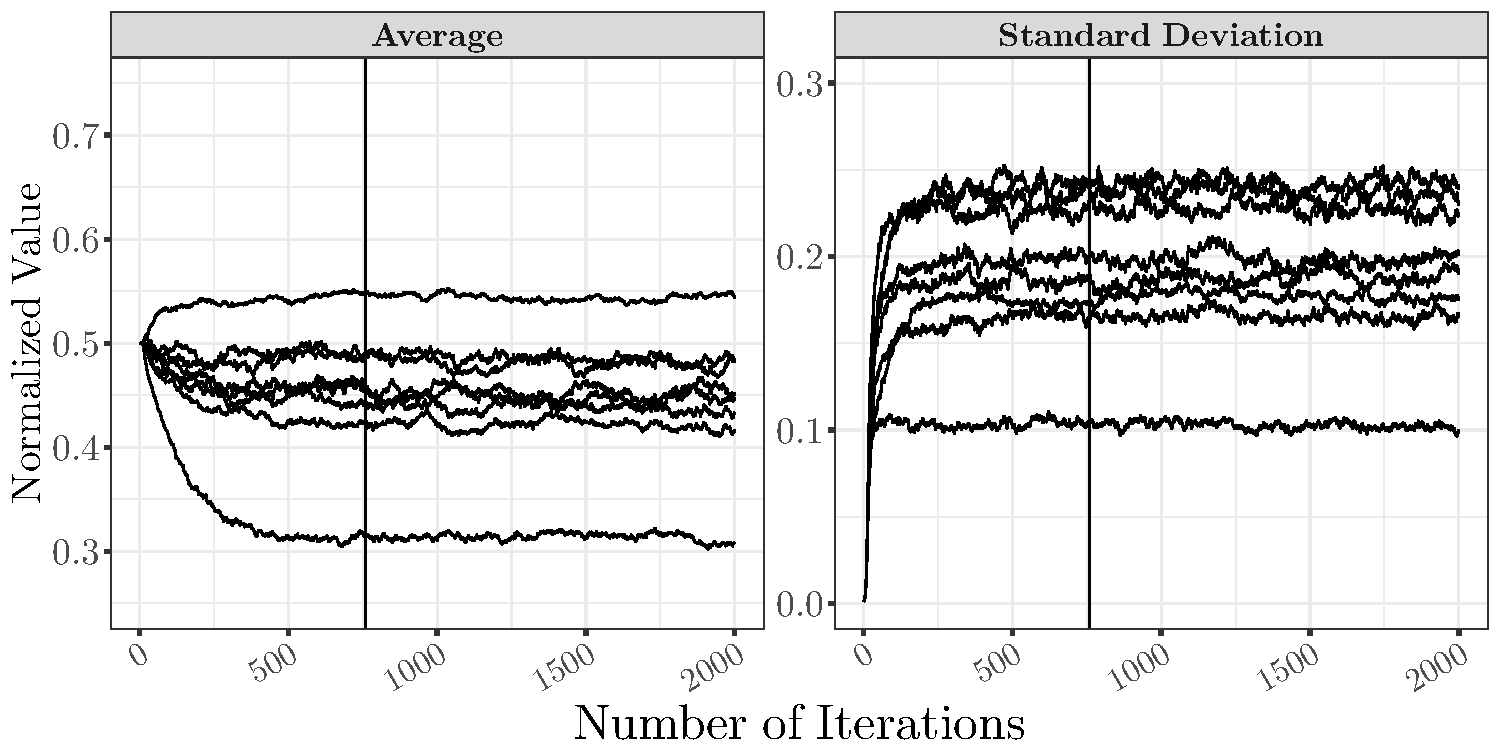
\includegraphics[width=1.0\textwidth]{../figures/chapter5/figures/plotEnsStatMCMC}
    \caption[Ensemble average and standard deviation as function of the number of iterations for calibration with model bias term.]{Ensemble average and standard deviation as function of the number of iterations for calibration with model bias term. Vertical lines indicate the iterations for burn-in (i.e., approximately $10$ times the autocorrelation time).}
    \label{fig:ch5_plot_ens_stat_mcmc}
\end{figure}

\begin{table}[h]
	\myfloatalign
	\caption[Estimated autocorrelation times for the $8$ model parameters with respect to the ensemble running average and standard deviation, for the calibration with model bias term.]{Estimated autocorrelation times for the $8$ model parameters with respect to the ensemble running average and standard deviation, for the calibration with model bias term. The bold term indicates the largest autocorrelation time used to determine the length of burn-in.}
	\label{tab:ch5_ens_stat_mcmc}
	\begin{tabularx}{1.05\textwidth}{rlccccc} \toprule
		\multirow{2}{*}{No.}&\multirow{2}{*}{Parameter}		&\multicolumn{2}{c}{Average}	&\phantom{a}&\multicolumn{2}{c}{Standard Deviation}\\
																												\cmidrule{3-4}	                           \cmidrule{6-7}
      &												& $\tau_{\text{pre-burn-in}}$ 	& $\tau_{\text{post-burn-in}}$	&& $\tau_{\text{pre-burn-in}}$ & $\tau_{\text{post-burn-in}}$ \\ \midrule
		\footnotesize{1}	&	\footnotesize{\texttt{gridHT}	}			  & \footnotesize{$64.3$}  				& \footnotesize{$6.8$} 	        && \footnotesize{$30.1$}  		 & \footnotesize{$26.6$}\\
		\footnotesize{2}	&	\footnotesize{\texttt{iafbWHT}} 			& \footnotesize{$31.6$} 				& \footnotesize{$22.5$} 	      && \footnotesize{$24.3$}  		 & \footnotesize{$21.8$}\\
		\footnotesize{3}	&	\footnotesize{\texttt{dffbWHT}} 			& \footnotesize{$51.1$}  				& \footnotesize{$29.9$} 	      && \footnotesize{$16.7$}  		 & \footnotesize{$16.8$}\\
		\footnotesize{4}	&	\footnotesize{\texttt{dffVIHT}}			  & \footnotesize{$66.3$}  				& \footnotesize{$22.3$} 	      && \footnotesize{$28.2$}  		 & \footnotesize{$14.4$}\\
		\footnotesize{5}	&	\footnotesize{\texttt{iafbIntDr}} 		& \footnotesize{$57.6$}  				& \footnotesize{$38.8$} 	      && \footnotesize{$21.8$}  		 & \footnotesize{$15.9$}\\
		\footnotesize{6}	&	\footnotesize{\texttt{dffbIntDr}} 		& \footnotesize{$\bm{75.5}$}  	& \footnotesize{$17.5$} 	      && \footnotesize{$18.5$}  		 & \footnotesize{$22.7$}\\
		\footnotesize{7}	&	\footnotesize{\texttt{dffbWDr}}			  & \footnotesize{$27.1$}  				& \footnotesize{$18.7$} 	      && \footnotesize{$50.1$}  		 & \footnotesize{$6.5$}\\
		\footnotesize{8}	&	\footnotesize{\texttt{tQuench}} 			& \footnotesize{$53.4$}  				& \footnotesize{$13.1$} 	      && \footnotesize{$28.2$}  		 & \footnotesize{$16.0$}\\
		\bottomrule
	\end{tabularx}
\end{table}
